\documentclass[11pt,a4paper]{article}

\usepackage[utf8]{inputenc} 
\usepackage[T1]{fontenc} 
\usepackage{lmodern}
\usepackage[margin=2cm]{geometry}
\usepackage[german]{babel}
\usepackage{amsmath} 
\usepackage{graphicx} 
\usepackage{booktabs}
\usepackage{hyperref}
\usepackage{mathtools}
\hypersetup{
    colorlinks,
    citecolor=red,
    filecolor=black,
    linkcolor=black!20!blue!90!,
    urlcolor=black} 
\usepackage{nicefrac}
\usepackage[table]{xcolor}
\usepackage{tocloft}

\setlength{\parindent}{0pt}
\setlength{\parskip}{1ex plus 0.5ex minus 0.5ex}

\definecolor{incolor}{rgb}{0.0, 0.0, 0.5}

\hbadness=99999

\newcommand{\refpy}[1]{Siehe Anhang: \textit{Rechnungen in Python} (\texttt{{\color{incolor}In [{\color{incolor}#1}]}})}
\newcommand\dif{\mathop{}\!\mathrm{d}}
\newcommand{\halftime}[4]{\begin{figure}[h]
\begin{minipage}{.#1\textwidth}#3\end{minipage}\begin{minipage}{.#2\textwidth}
\centering
#4\end{minipage}
\end{figure}}
\renewcommand{\vec}{\boldsymbol}

\begin{document}

{
\centering 
\large 
Physiklabor für Anf\"anger*innen \\
Ferienpraktikum im Sommersemester 2018 \\[4mm]
\textbf{\LARGE 
Versuch 06: Elastizitätskonstante
} \\[3mm]
(durchgef\"uhrt am 24.09.2018 bei Julia Müller) \\
Andréz Gockel, Patrick M\"unnich\\
\today \\[10mm]
}

\vspace{50pt}
\tableofcontents
\vspace{22pt}
\listoftables
\vspace{22pt}
\listoffigures
\pagebreak
\phantom{lol}
\pagebreak

\section{Ziel des Versuchs}

Das Ziel des Versuchs ist es, den Elastizit\"atsmodul von drei unterschiedlichen isotropen Festk\"orpern mittels Biegung zu ermitteln. Au\ss erdem soll die Abh\"angigkeit der Biegung eines Stabes mit rechteckigen Querschnitt vom Material, der Ausrichtung und der L\"ange untersucht werden.

\section{Teil XX}

\subsection{Theorie}

Wird eine (nicht all zu gro\ss e) Kraft $F$ auf einen elastischen Festk\"orper ausge\"ubt, so f\"uhrt dies zu einer L\"angen\"anderung $\Delta l$. F\"ur hinreichend kleiner Kr\"afte ist die L\"angen\"anderung proportional zur angreifenden Kraft. Den Kehrwert dieser Proportionalit\"atskonstante wird als Elastizit\"atsmodul $E$ bezeichnet (\textit{Hooke}'sches Gesetz):

\begin{equation}
\frac{\Delta l}{l}=\frac{F}{EA}=\frac{\sigma}{E}\label{eq:elast}
\end{equation}

Wie in Abbildung \ref{Abb:1} zu erkennen, f\"uhrt die Biegung eines Balkens zu Stauchung und Streckung oberhalb und unterhalb der sog. \textit{neutralen Faser}.

\begin{figure}[h]
\centering
\fbox{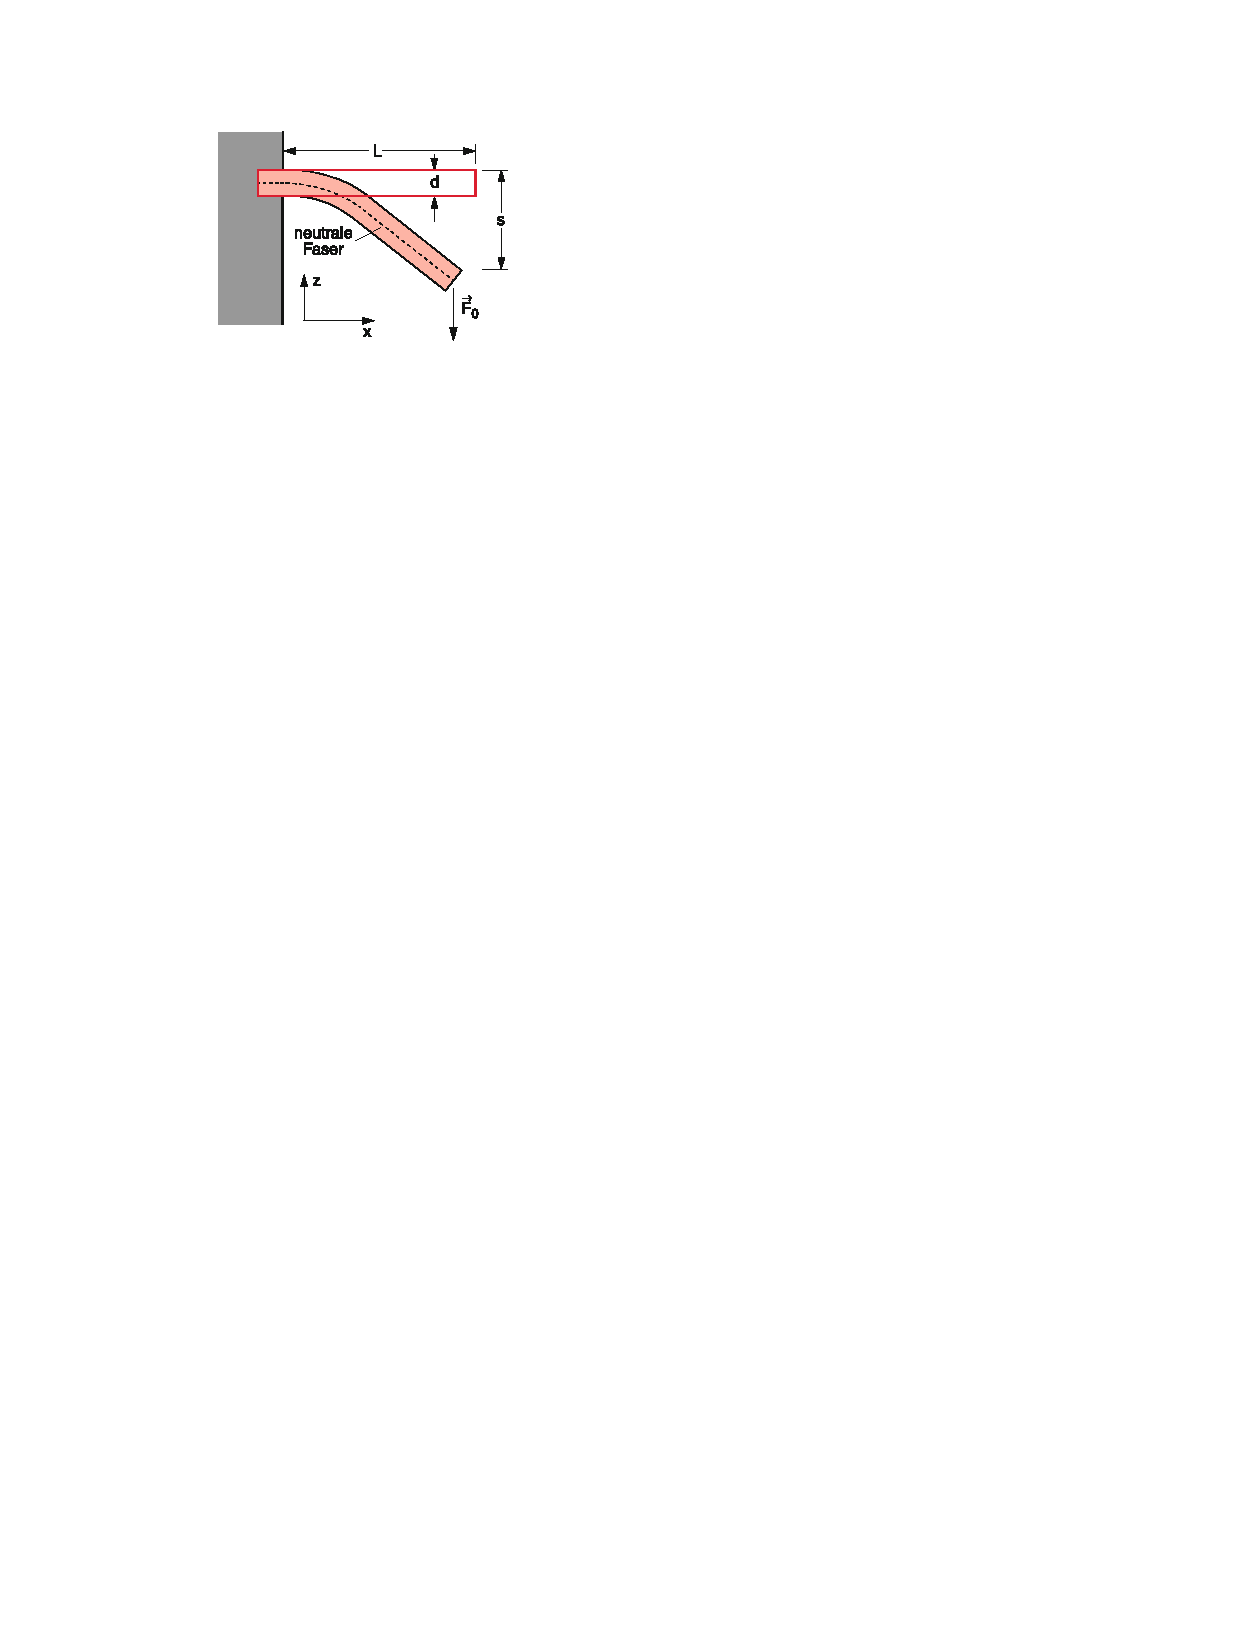
\includegraphics[width=0.8\textwidth]{neutraleFaser.pdf}}
\renewcommand\thefigure{1}
\caption[Biegung eines Stabes unter Einfluss einer Kraft $F_0$ mit neutraler Faser]{Biegung eines Stabes unter Einfluss einer Kraft $F_0$ mit neutraler Faser \cite{Demtr\"oder}}
\label{Abb:1}
\end{figure}

\pagebreak

Nach dem \textit{Hooke}'schen Gesetz ist diese Biegung/Stauchung f\"ur kleine Gewichte proportional zur angreifenden Kraft. F\"ur einen Balken, der an beiden Enden unterst\"utzt wird (Abbildung \ref{Abb:2}), ergibt sich

\begin{equation}
s\mathrel{:\mkern-0.25mu=} z(x=\nicefrac{l}{2})=\frac{1}{E}\frac{l^3}{4h^3b}F\label{eq:biegp}
\end{equation}

\begin{figure}[h]
\centering
\fbox{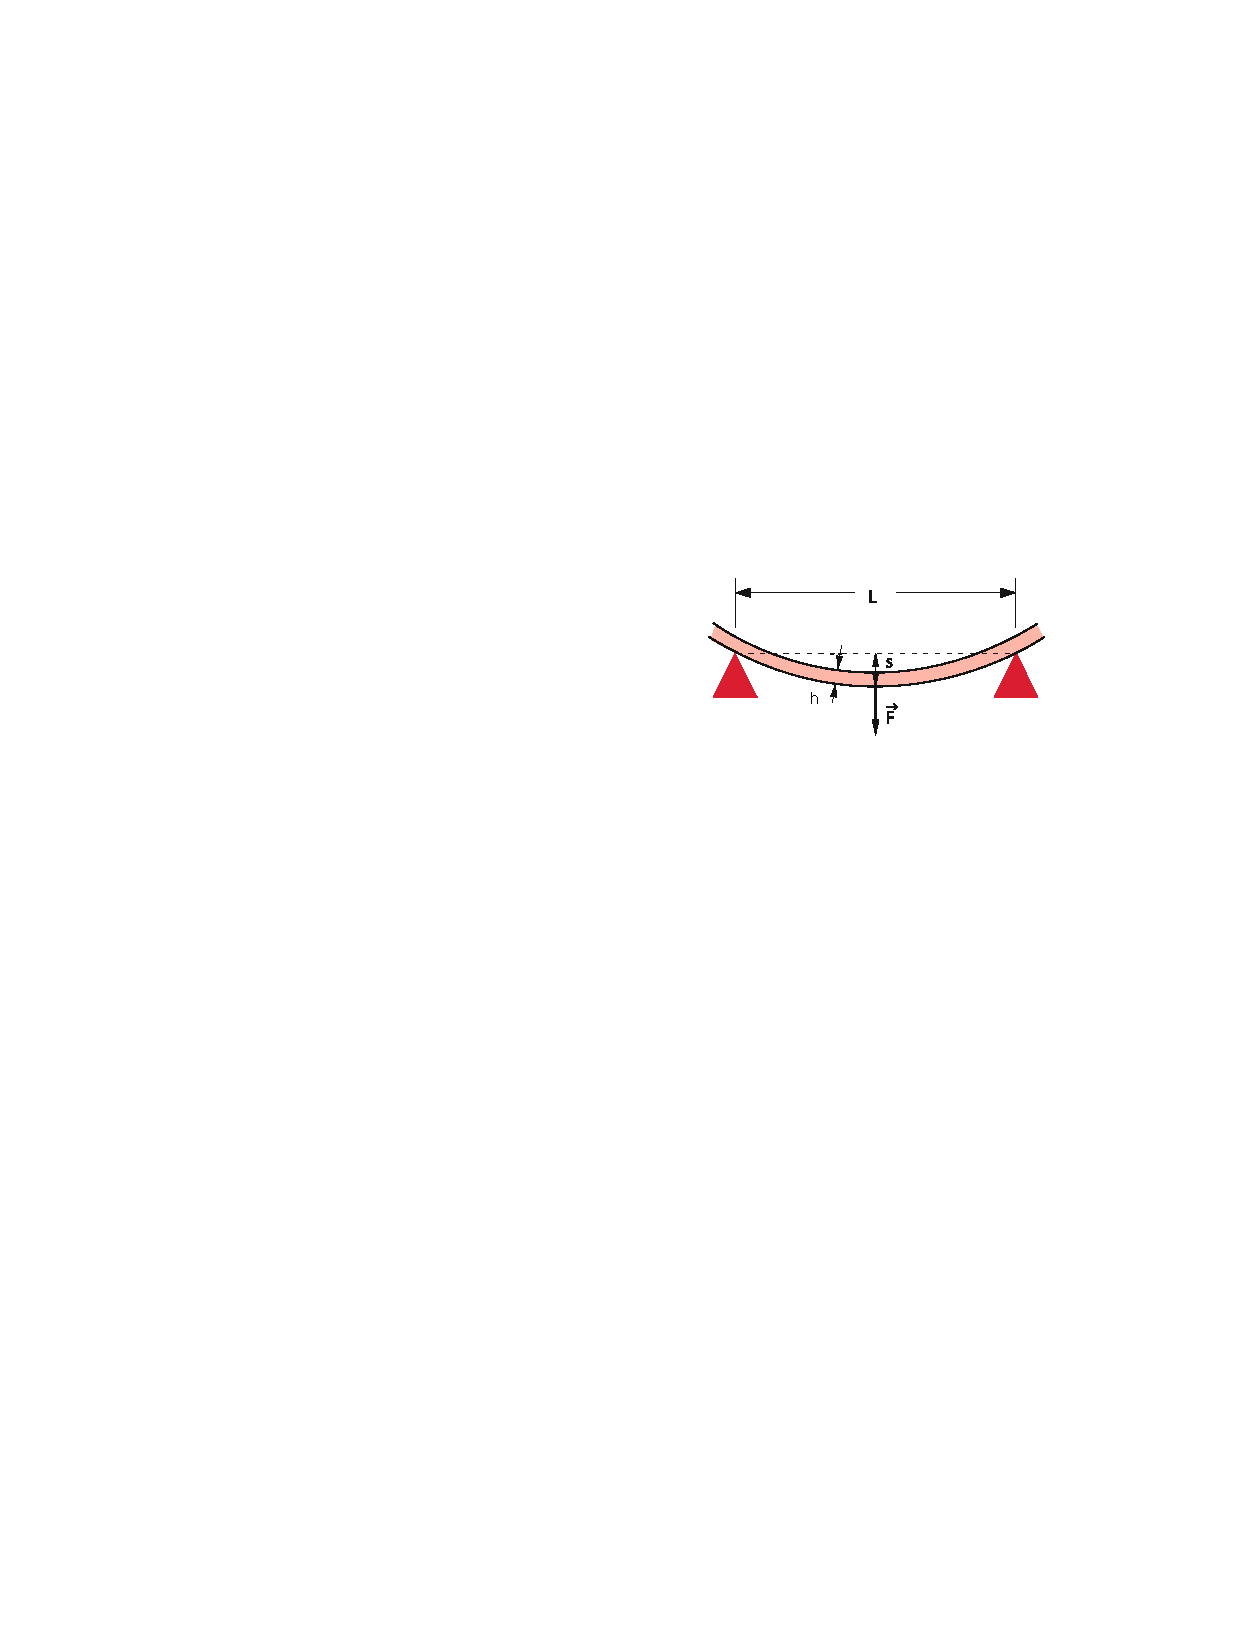
\includegraphics[width=0.8\textwidth]{versuchsaufbau.pdf}}
\renewcommand\thefigure{2}
\caption[Versuchsaufbau]{Versuchsaufbau \cite{Demtr\"oder}}
\label{Abb:2}
\end{figure}

\subsection{Aufbau}

% describe set up
% insert pic name, designation, toc caption, caption, label
%\halftime{5}{5}{TEXT}{\fbox{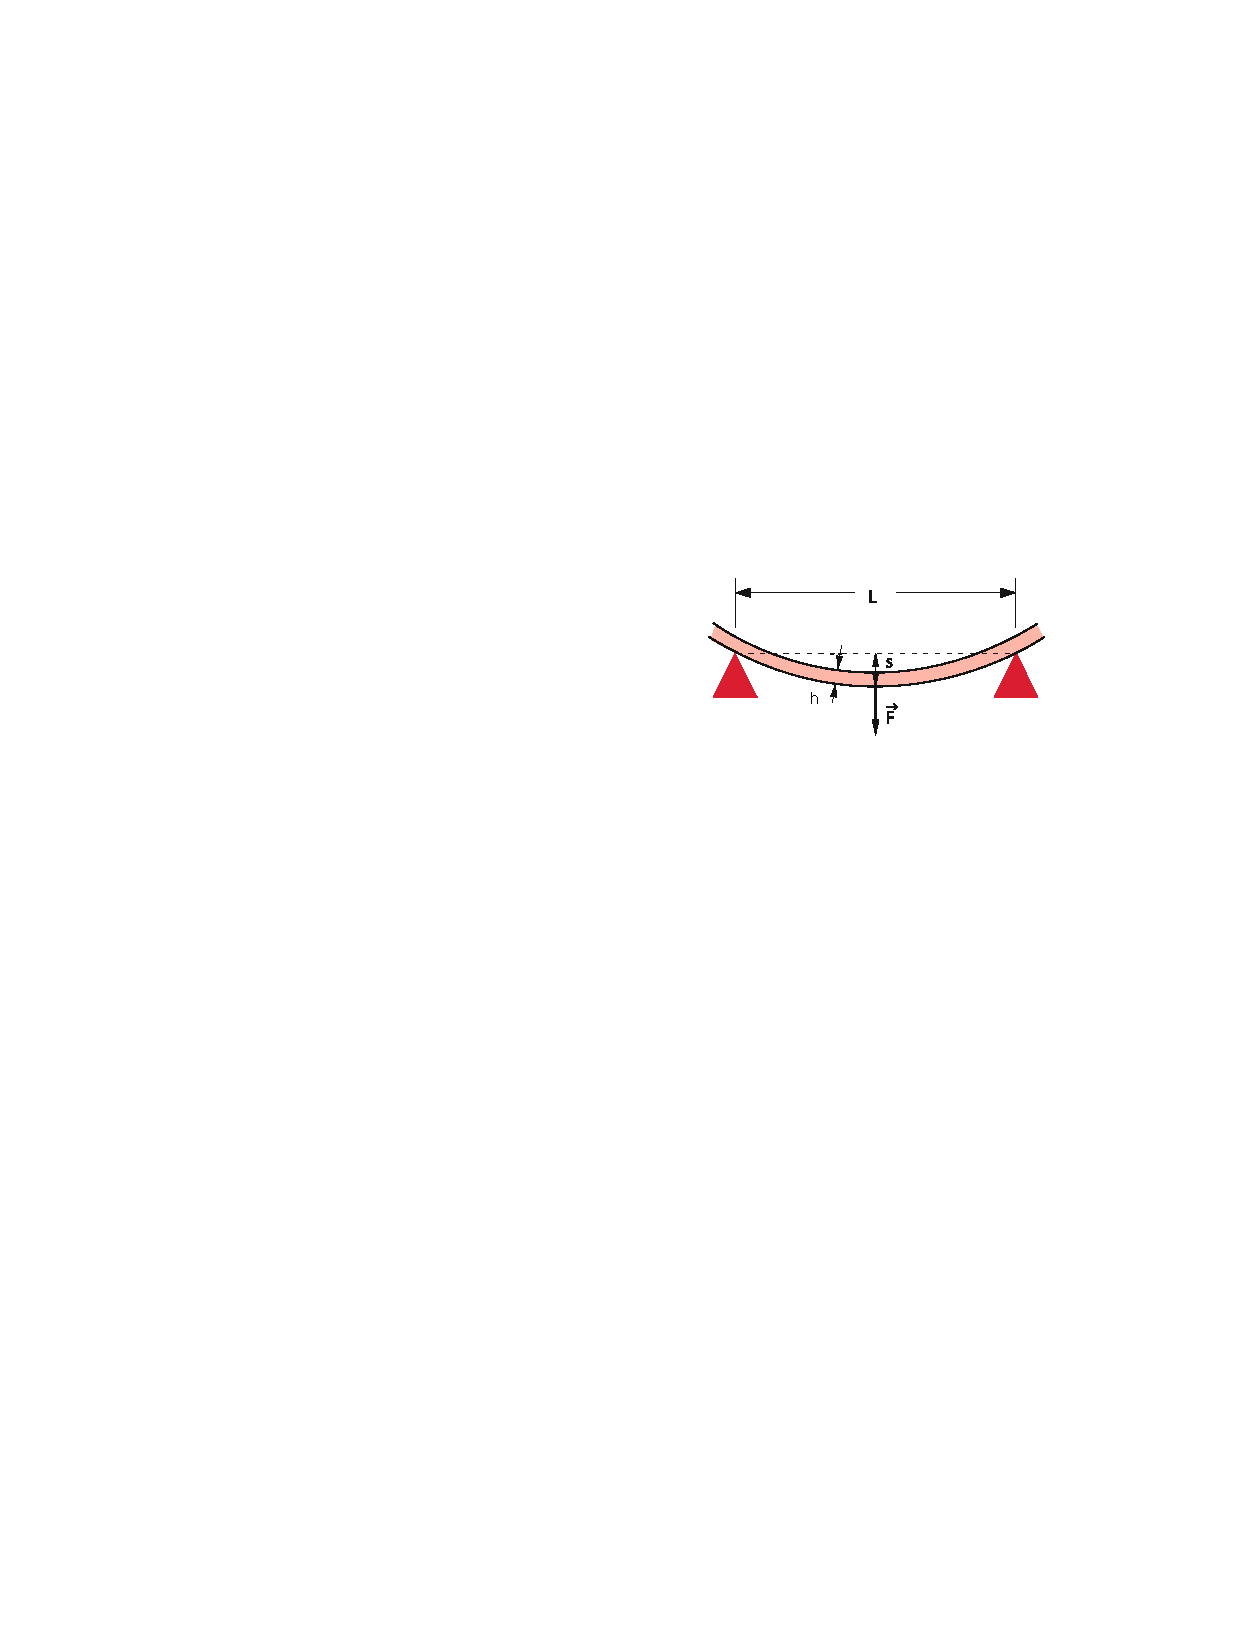
\includegraphics[width=0.8\textwidth]{versuchsaufbau.pdf}}
%   \renewcommand\thefigure{BX}
%\caption[XXXX]{XXXX \cite{Anleitung}}
%\label{Pic:X}}

\subsection{Durchführung}

% describe exp.
XXXX

\subsection{Auswertung}




\section{Diskussion}

Es wirken noch zus\"atzliche Kr\"afte, welche durch das Eigengewicht der St\"abe, das Gewicht der Halterung und der Andruckkraft des Messger\"ats ausge\"ubt werden. Da dieser Versuch sich aber im Proportionalit\"atsbereich aufh\"alt, m\"ussen diese Kr\"afte nicht ber\"ucksichtigt werden, da sie nur den Nullpunkt des Messger\"ats verschieben.

\pagebreak

\section{Anhang: Tabellen und Diagramme}

\begin{table}[h]
\centering
\caption{XXXX} \vspace{11pt}
$\begin{array}{l}
\textrm{Unsicherheiten:}\\
\textrm{XXXX: } \pm XX \textrm{XX}\\
\end{array}$
\begin{tabular}{ccc}
\toprule
\textrm{XXXX}/\textrm{XX} & \textrm{XXXX}/\textrm{XX} & \textrm{XXXX}/\textrm{XX} \\
\midrule 
2 & 0.26 & 0.23\\
\hline
4 & 0.33 & 0.25\\
\hline 
5 & & 0.3\\
\hline 
6 & 1.25 & 0.83\\
\hline 
8 & 3.9 & 0.83\\ 
\hline
9 & 4.75 & 4.6\\ 
\hline
10 & 4.7 &\\ 
\bottomrule
\end{tabular}
\phantom{$\begin{array}{l}
\textrm{Unsicherheiten:}\\
\textrm{XXXX: } \pm XX \textrm{XX}\\
\end{array}$}
\label{Tab:X}
\end{table}

%\begin{figure}[p]
%\centering
%\fbox{\includegraphics[width=0.8\textwidth]{NAME}}
%\renewcommand\thefigure{BX}
%\caption[XXXX]{XXXX}
%\label{Abb:X}
%\end{figure}

\begin{thebibliography}{9}
\bibitem{Uncertainties}''Correlations between variables are automatically handled, which sets this module apart from many existing error propagation codes.'' - \url{https://pythonhosted.org/uncertainties/}
\bibitem{Anleitung} Physikalisches Institut der Albert-Ludwigs-Universität Freiburg (Hrsg.) (08/2018): Versuchsanleitungen zum Physiklabor für Anfänger*innen, Teil 1, Ferienpraktikum im Sommersemester 2018.
\bibitem{Demtr\"oder} Demtr\"oder, Experimentalphysik 1, \url{https://www.springer.com/us/book/9783662464151}, Kapitel 6.2.4
\end{thebibliography}

\end{document}